\documentclass[twoside]{article}
\usepackage{aistats2014}

\usepackage{times}

%\newtheorem{observation}{Observation}
%\newtheorem{claim}{Claim}
%\newtheorem{conjecture}{Conjecture}
%\newtheorem{problem}{Problem}
%\newtheorem{algo}{Algorithm}
%\newtheorem{definition}{Definition}
%\newtheorem{lemma}{Lemma}
%\newtheorem{theorem}{Theorem}
%\newtheorem{proof}{Proof}
%\newtheorem{defi}{Definition}

\newcommand\independent{\protect\mathpalette{\protect\independenT}{\perp}}
\def\independenT#1#2{\mathrel{\setbox0\hbox{$#1#2$}%
\copy0\kern-\wd0\mkern4mu\box0}} 

\newcommand{\atiter}[2]{{#1}^{(#2)}}
\newcommand{\itert}[1]{{#1}^{(t)}}
\newcommand{\itertO}[1]{{#1}^{(t+1)}}
\newcommand{\iiter}[1]{{#1}^{(i)}}
% \newcommand{\raiseTheta}[1]{\theta^{#1}}
\newcommand{\raisePsi}[1]{\psi^{#1}}
\newcommand{\order}[1]{\mathcal{O}(#1)}

\newcommand{\hide}[1]{}
\newcommand{\comment}[1]{\textcolor{red}{{\small #1 }}}
\newcommand{\semihide}[1]{{\tiny #1}}
\newcommand{\reminder}[1]{{\textsf{\textcolor{red}{[#1]}}}}
\newcommand{\makeclean}{
    \renewcommand{\reminder}[1]{}
}

%\newcommand{\QED}{ \hfill {\bf QED}}
\newcommand{\tight}{ \setlength{\itemsep}{-1.0\itemsep} }
    % makes lists tighter

\usepackage[mathscr]{eucal} %% For \mathscr
\usepackage{amsbsy} %% For \boldsymbol
\newcommand{\tensor}[1]{\boldsymbol{\mathscr{#1}}}   %% Tensor macro from Tammy
% \newcommand{\tensor}[1]{{\boldmath\mathcal{#1}}}
\newcommand{\B}[1]{\mathbf{#1}}   %% Tensor macro from Tammy
%\newcommand{\tensor}[1]{\underline{\mathbf{#1}}}  
%\newcommand{\tensor}[1]{\mathbf{\EuScript{#1}}}  
%\newcommand{\tensor}[1]{\mathbf{\mathcal{#1}}}  
\newcommand{\loss}{\mathcal{L}}  

\newcommand{\krp}[2]{ \left( \mathbf{#1}\odot\mathbf{#2} \right)}

\def\blambda{\mbox{\boldmath ${\lambda}$}}

\newcommand{\method}{\textsc{METHOD}\xspace}
\newcommand{\methodplain}{METHOD\xspace}
\newcommand{\graphlab}{GraphLab\xspace}
\newcommand{\psgd}{PSGD\xspace}
\newcommand{\dsgd}{DSGD+\xspace}
\newcommand{\lda}{LDA\xspace}
\newcommand{\dl}{DL\xspace}
\newcommand{\mmsb}{MMSB\xspace}
\newcommand{\twitter}{TGraph\xspace}
\newcommand{\nytimes}{NyTimes\xspace}
\newcommand{\snytimes}[1]{NyTimes{#1}\xspace}
\newcommand{\scaleblenytimes}{Scalable NyTimes\xspace}
\newcommand{\pubmed}{PubMed\xspace}
\newcommand{\imagenet}{ImageNet\xspace}

\newcommand{\sgd}{SGD\xspace}

%\newcommand{\explosion}{\textsc{Idex}\xspace}
\newcommand{\explosion}{intermediate data explosion\xspace}
\newcommand{\Explosion}{Intermediate Data Explosion\xspace}
\newcommand{\gtscaleup}{100\xspace}

\newcommand{\samplecube}{\textsc{ParCube}\xspace}
\newcommand{\parafac}{\textsc{Parafac}\xspace}
\newcommand{\sparafac}{\textsc{Parafac SLF}\xspace}
\newcommand{\merge}{\textsc{Merge}\xspace}
\newcommand{\sample}{\textsc{BiasedSample}\xspace}
\newcommand{\enron}{\textsc{Enron}\xspace}
\newcommand{\facebook}{\textsc{Facebook}\xspace}
\newcommand{\lbnl}{\textsc{Lbnl}\xspace}
\newcommand{\nell}{\textsc{Nell}\xspace}
\newcommand{\argmin}{\text{argmin}\xspace}
\newcommand{\brain}{\textsc{BrainQ}\xspace}


\newcommand{\hadi}{{\cal HADI}\xspace}
\newcommand{\mapreduce}{\textsc{MapReduce}\xspace}
\newcommand{\map}{\textsc{Map}\xspace}
\newcommand{\reduce}{\textsc{Reduce}\xspace}
\newcommand{\combine}{\textsc{Combine}\xspace}
\newcommand{\hadoop}{\textsc{Hadoop}\xspace}
\newcommand{\anf}{\emph{Centralized Method}}
% \newcommand{\MFB}{{MF-bitstring}}
\newcommand{\MFB}{{FM-bitstring}}
\newcommand{\mfb}{{b}}
\newcommand{\MFV}{{FM-vector}}
\newcommand{\mfv}{{\bf v}}
% \newcommand{\mfbhi}{{MF-vector}}
\newcommand{\mfbhi}{{ b(h,i) }}
\newcommand{\Nhi}{N(h,i)}   % number of neighbors of $i$, within h hops or less
\newcommand{\NNhi}{ {\cal N}(h,i)} % SET of neighbors ....
\newcommand{\NNhhi}{ {\cal N}(h+1,i)} % SET of neighbors ....
\newcommand{\NNhj}{ {\cal N}(h,j)} % SET of neighbors ....
\newcommand{\hatmfbhi}{ $\hat{b}(h,i)$} %partial bitmask

\newcommand{\PassA}{{\tt Stage1}\xspace}
\newcommand{\PassAMap}{{\tt Stage1-Map}\xspace}
\newcommand{\PassARed}{{\tt Stage1-Reduce}\xspace}
\newcommand{\PassB}{{\tt Stage2}\xspace}
\newcommand{\PassBMap}{{\tt Stage2-Map}\xspace}
\newcommand{\PassBRed}{{\tt Stage2-Reduce}\xspace}
\newcommand{\PassC}{{\tt Stage3}\xspace}
\newcommand{\PassCMap}{{\tt Stage3-Map}\xspace}
\newcommand{\PassCRed}{{\tt Stage3-Reduce}\xspace}

\newcommand{\diameter}{{\tt diameter}}
\newcommand{\npairs}{{\tt npairs}}
\newcommand{\gcc}{{\tt gcc}}
\newcommand{\entropy}{{\tt entropy}}
% \newcommand{\nedges}{{\tt nedges}}
\newcommand{\sv}{{\mbox{$\lambda_1$}}}
\newcommand{\avgd}{{\tt avgd}}

% math symbol definitions
\newcommand{\mat}[1]{{\bf{#1}}}
\newcommand{\nnodes}{N}     % number of nodes
\newcommand{\nedges}{E}     % number of edges
\newcommand{\deff}{{d_{eff}}}   % effective diameter
\newcommand{\Er}{{E_{r}}}   % number of retained edges
\newcommand{\Nr}{{N_{r}}}   % number of retained nodes
\newcommand{\Nc}{{N_c}}   % number of nodes at critical point
\newcommand{\Ec}{{E_c}}   % number of nodes at critical point
\newcommand{\Ngcc}{{N_{gcc}}} % number of nodes in gcc, at critical poing
\newcommand{\NPairc}{{N_{NPAIRS}}} % number of reachable pairs, at critical poing
\newcommand{\dc}{{d_{c}}} % diameter at critical point
\newcommand{\Lambdac}{{\lambda_{c}}} % First eigenvalue at critical point
% \newcommand{\RED}{ {\em RED } } % random edge deletion
% \newcommand{\FED}{ {\em FED } } % friendly edge deletion
% \newcommand{\HED}{ {\em HED } } % hostile edge deletion
\newcommand{\join}{\texttt{combine2}}
\newcommand{\aggrnp}{\texttt{combineAll}}
\newcommand{\aggr}{\texttt{combineAll$_i$}}
\newcommand{\aggrsid}{\texttt{combineAll$_{E.sid}$}}
\newcommand{\assign}{\texttt{assign}}



\newcommand{\ben}{\begin{enumerate*}}
\newcommand{\een}{\end{enumerate*}}
\newcommand{\bit}{\begin{itemize*}}
\newcommand{\eit}{\end{itemize*}}

% shorthands
\newcommand{\citationsds}{{CITATIONS}}
\newcommand{\epinionsds}{{EPINIONS}}
\newcommand{\patentsds}{{PATENTS}}
\newcommand{\net}[1]{{\textsc{#1}}}

\newcommand{\QED}{\hfill $\Box$ \hfill}





% graph segment
% Notation macros
\newcommand{\G}{\ensuremath{{\mathcal G}}}  % graph stream
\newcommand{\ES}[1]{\ensuremath{m^{(\!#1\!)}}}
%\newcommand{\ES}[1]{\ensuremath{|E|^{(\!#1\!)}}}
\newcommand{\coll}{\ensuremath{\ell}}  % number of source/row groups
\newcommand{\rowk}{\ensuremath{k}}  % number of dest/col groups
\newcommand{\rgrp}[1]{\ensuremath{I^{(\!#1\!)}}}  % node set for src/row group
\newcommand{\cgrp}[1]{\ensuremath{J^{(\!#1\!)}}} % node set for dst/col group
\newcommand{\rgsz}[1]{\ensuremath{l^{(\!#1\!)}}}  % size of node set for src/row group
\newcommand{\cgsz}[1]{\ensuremath{n^{(\!#1\!)}}  }% size of node set for dst/col group
\newcommand{\subG}[1]{\ensuremath{{\mathcal G}^{(\!#1\!)}}}  % submatrices
\newcommand{\den}[1]{\ensuremath{\rho^{(\!#1\!)}}}   % density/probability
\newcommand{\KL}[2]{\ensuremath{{\mathcal D}(#1\|#2)}}   % KL-divergence
\newcommand{\ceil}[1]{\ensuremath{\lceil\!#1\!\rceil}}   % density/probability

\newcommand{\myrot}[1]{\rotatebox[origin=ll]{75}{{#1}}} 


\usepackage{amsmath,amsfonts,amssymb}
\usepackage{subfigure,grffile,placeins}
\usepackage{graphicx} 
\usepackage{epstopdf}
\usepackage{hyperref}
\usepackage{wrapfig}
\usepackage[lined,boxed]{algorithm2e}
\usepackage{url}
%\usepackage{color}
\usepackage{xcolor}

\newtheorem{observation}{Observation}
\newtheorem{conjecture}{Conjecture}
\newtheorem{problem}{Problem}
\newtheorem{algo}{Algorithm}
\newtheorem{definition}{Definition}
\newtheorem{lemma}{Lemma}
\newtheorem{theorem}{Theorem}
\newtheorem{assumption}{Assumption}
%\newtheorem{question}{Question}
\newtheorem{example}{Example}
\newcommand{\pushright}[1]{\ifmeasuring@#1\else\omit\hfill$\displaystyle#1$\fi\ignorespaces}
\newcommand{\pushleft}[1]{\ifmeasuring@#1\else\omit$\displaystyle#1$\hfill\fi\ignorespaces}
%\newtheorem{answer}{Answer}
%\newtheorem{proof}{Proof}
\newcommand{\psgd}{PSGD\xspace}
\newcommand{\dsgd}{DSGD+\xspace}
\newcommand{\lda}{LDA\xspace}
\newcommand{\dl}{DL\xspace}
\newcommand{\sdl}{SDL\xspace}
\newcommand{\mmsb}{MMSB\xspace}
\newcommand{\webgraph}{WebGraph\xspace}
\newcommand{\nytimes}{NyTimes\xspace}
\newcommand{\snytimes}[1]{NyTimes{#1}\xspace}
\newcommand{\scaleblenytimes}{Scalable NyTimes\xspace}
\newcommand{\pubmed}{PubMed\xspace}
\newcommand{\imagenet}{ImageNet\xspace}
\newcommand{\model}{model\xspace}
\newcommand{\data}{data\xspace}

\newcommand{\sgd}{SGD\xspace}

\newcommand{\abhi}[1]{\textcolor{orange}{abhi-comment: #1}}
\newcommand{\alex}[1]{\textcolor{red}{alex-comment: #1}}
\newcommand{\qirong}[1]{\textcolor{magenta}{qirong-comment: #1}}
\newcommand{\eric}[1]{\textcolor{blue}{[Eric-comment: #1]}}

\newcommand{\ourmethod}{FlexiLearn}

% If your paper is accepted, change the options for the package
% aistats2014 as follows:
%
%\usepackage[accepted]{aistats2014}
%
% This option will print headings for the title of your paper and
% headings for the authors names, plus a copyright note at the end of
% the first column of the first page.

\begin{document}

% If your paper is accepted and the title of your paper is very long,
% the style will print as headings an error message. Use the following
% command to supply a shorter title of your paper so that it can be
% used as headings.
%
%\runningtitle{I use this title instead because the last one was very long}

% If your paper is accepted and the number of authors is large, the
% style will print as headings an error message. Use the following
% command to supply a shorter version of the authors names so that
% they can be used as headings (for example, use only the surnames)
%
%\runningauthor{Surname 1, Surname 2, Surname 3, ...., Surname n}

\twocolumn[

\aistatstitle{Slow-Worker-Agnostic Distributed Learning for Big Models on Big Data}

%\aistatsauthor{Abhimanu Kumar \And Alex Beutel 2 \And Qirong Ho \And Eric P. Xing}
\aistatsauthor{Anonymous Authors}
\aistatsaddress{ Unknown Institution} ]

\begin{abstract}
We present a scheme for fast, distributed learning on
big (i.e. high-dimensional) models applied to big datasets.
Unlike algorithms that focus on distributed learning in either the big data or big model setting
(but not both), our scheme partitions both the data and model variables
simultaneously. This not only leads to faster learning on distributed clusters,
but also enabes machine learning applications where both data
and model are too large to fit within the memory of a single machine. Furthermore, our scheme
allows worker machines to perform additional updates while waiting for slow workers to finish,
which provides users with a tunable synchronization strategy that can
be set based on learning needs and cluster conditions.
We prove the correctness of such strategies, as well as provide
bounds on the variance of the model variables under our scheme.
Finally, we present empirical results for latent space models such
as topic models, which demonstrate that our method
scales well with large data and model sizes, while beating
learning strategies that fail to take both data and model partitioning into account.
\end{abstract}

\vspace{-0.3cm}
\section{Introduction}
\vspace{-0.2cm}

Machine Learning applications continue to grow rapidly, in terms of both input
data size (big data) as well as model complexity (big models). The big data challenge
is already well-known --- with some estimates putting the amount of data generated on the internet
at 5 exabytes every two days~\footnote{\scriptsize\url{http://techcrunch.com/2010/08/04/schmidt-data/}} ---
and much effort has been devoted towards learning models on big datasets, particularly through
stochastic optimization techniques that randomly partition the data over different machines. Such techniques
have been the subject of much theoretical
scrutiny~\cite{langford2009slow,zinkevich2010parallelized,agarwal2012distributed,hoffman2012stochastic}.
On the other hand, the big model issue, which is about learning models with an extremely large number of variables
and/or parameters --- such as the Google Brain deep network with over 1B parameters~\cite{dean2012large} --- has just started to gain greater attention,  
and recent papers on this subject have primarily focused on intelligent partitioning of the model variables in
order to minimize network synchronization costs~\cite{low2012distributed,dean2012large}, albeit not always
with theoretical backing.

Although big data and big models are both crucial research foci, there are few
distributed machine learning efforts that explicitly consider both aspects in conjunction, with a notable example
being the partitioned matrix factorization algorithm of Gemulla {\it et al.}~\cite{Gemulla:2011:LMF:2020408.2020426}, which
divides the input matrix $X$ into independent blocks that do not overlap on rows or columns --- thus allowing the factors $AB=X$
to be updated correctly in parallel.
%\eric{add a sentence here to describe the work.}.
More generally, in the big data,
big model setting, the model variables may not all fit into a single machine's memory, which in turn imposes
additional constraints on how the data is partitioned. Furthermore, careless partitioning of model variables
across distributed machines imposes significant network synchronization costs~\cite{low2012distributed}, which
are required whenever dependent variables or datapoints are placed on separate machines.
If we are to effectively partition both data and model, it follows that we must carefully
examine and exploit the interdependencies between data and model variables.

In this paper, we investigate the theoretical and algorithmic challenges for learning large-scale latent space models on big data over a distributed cluster.
We develop and analyze a stochastic optimization approach for learning latent space models expressed in a matrix form, such as topic modeling or dictionary learning. Our proposed algorithm, {\it \ourmethod},
%\eric{it would be nice to have a name XXX for our algorithm here.}
exploits the structures of the model in question to partition the input data and model variables over the cluster, in a manner that automatically balances inter-machine network synchronization costs with performing useful computational work, even when the worker machines are not equally capable (e.g. because of different hardware or other
concurrently running programs), or the data cannot be evenly partitioned (e.g. due to the dependency structure of the model).

\ourmethod~solves the ``last reducer" or ``straggler" issue in distributed systems, in which some worker machines can be much slower than others (because of cluster heterogeneity, or because other jobs are running on the same machine), causing faster workers to waste computational cycles waiting for them.
Instead, our algorithm ensures that the faster workers will continue to perform useful work until the last reducer finishes --- and if the last reducer
is unable to finish, it can be restarted without affecting program correctness, while the faster workers continue doing work.
%\eric{what if that reducer never finishes, or is extremely slow?}
Beacuse \ourmethod~has modest synchronization and communication requirements, it
is easy to implement on top of common distributed computing systems such as Hadoop ---
yet it can also be applied to specialized systems for big Machine Learning, such as parameter
servers~\cite{ho2013more,cipar2013solving,ahmed2012scalable,power2010piccolo},
in order to further improve their performance.
Finally, our theoretical and empirical analysis confirms that \ourmethod~can provide faster convergence
on a variety of latent space problems in ML;
furthermore, careful control of inter-worker synchronization can lead to even faster convergence,
which opens the door to intelligent exploitation of fine-grained synchronization schemes (such
as the aforementioned parameter servers).

\vspace{-0.3cm}
\section{Related Work}
\vspace{-0.2cm}

Most existing literature is focused on learning under either big data or big model conditions, but
rarely both together. Of the papers that focus on big data, most of them exploit data point
indepedence to construct stochastic distributed optimization schemes with little need
for inter-machine synchronization. For example, the PSGD algorithm~\cite{zinkevich2010parallelized}
is completely data parallel and requires absolutely no inter-machine communication,
therefore making it trivial to implement. However, in practice,
one can almost always obtain faster convergence with some inter-machine communication, as our experiments will show.
Another important class of methods are the fixed-delay algorithms~\cite{agarwal2012distributed,langford2009slow} in which machines communicate
with a central server (or each other) in a fixed ordering. This fixed ordering is a serious practical limitation,
because all machines will be held up by slowdowns or failures in just one machine.
In contrast, our algorithm ensures that all machines continue to do useful work even under such conditions.
Most importantly, unlike these big data algorithms, our algorithm can partition model variables
(and not just datapoints) across machines, which is absolutely critical for massive models that cannot fit onto a single machine.

For learning on big models, the general strategy is to exploit the fact that each model variable usually
depends on only a small number of other variables, and then partition model variables
in a way that limits the number of dependencies that cross machines. The GraphLab system~\cite{low2012distributed}
is a good example of this concept, but it requires machine learning algorithms to be rewritten into
``vertex programs", which can be awkward or even difficult for some algorithms. Furthermore,
there has been little theoretical analysis on machine learning algorithms running under GraphLab.
The Google Brain project~\cite{dean2012large} provides another example of the need for model partitioning,
this time for a custom-built deep network meant for image and video feature extraction. However, the
paper does not provide general partitioning strategies for arbitrary models. Finally, we note that
the Hogwild paper~\cite{niu2011hogwild} provides a theoretical analysis of certain issues related to model partitioning ---
specifically, the effect of errors produced when two worker threads update the same variable simultaneously.
Aside from that, the paper does not provide or analyze model partitioning strategies, while their
experiments only cover the shared-memory, single-machine setting.

Finally, there are papers that tackle big data and big model issues together, such as the partitioned matrix factorization
algorithm of Gemulla {\it et al.}~\cite{Gemulla:2011:LMF:2020408.2020426}, to which our work is most closely related. Unlike Gemulla {\it et al.},
our algorithm allows worker machines to perform useful variable updates continuously, without blocking or waiting
for any other machine to complete its assigned task. This property is exceptionally beneficial
on very large clusters, where machines often fail or slow down for any number of reasons. Thus, our algorithm
is not bottlenecked by the slowest machine, unlike~\cite{Gemulla:2011:LMF:2020408.2020426}. Furthermore, we provide substantially
richer theoretical analysis, including variance bounds and analysis of the effect of non-blocking workers.
In particular, work by Murata~\cite{Murata98astatistical} lays the foundation for
variance analysis of SGD algorithms, by providing variance bounds over datapoint selection.

A special class of big ML systems are the parameter servers, which provide a distributed shared-memory interface
for large numbers of model parameters~\cite{ahmed2012scalable,power2010piccolo}, but perform no variable scheduling themselves.
Recent work on parameter
servers has led to new, theoretically-sound computational models such as Stale Synchronous Parallelism (SSP)~\cite{ho2013more,cipar2013solving},
which is fundamentally related to \ourmethod~in that both allow faster workers to perform additional work, without being
held up by slower workers. The main difference between SSP and \ourmethod~is that SSP is employed to reduce
inter-machine communication regardless of how updates are scheduled, whereas \ourmethod~is used to intelligently
schedule updates while assuming limited capacity for inter-machine communication. In future work, we intend to explore
how \ourmethod~and such computational models can be combined to tackle big data+model problems of even greater scale.

\vspace{-0.3cm}
\section{\ourmethod~--- Slow-Worker Agnostic Learning for Big Models on Big Data}
\vspace{-0.2cm}

The key principle behind \ourmethod~is to exploit independent or weakly-dependent blocks of data, variables and parameters.
For example, a probabilistic graphical model can contain many latent variables and parameters that capture the modeler's generative assumptions about large datasets. In order to tackle problems of such scale, we need to exploit independence structures present in the data and model, so as to partition both over a distributed cluster.

Before describing our partitioning strategy, we motivate our method with examples of popular latent space models recently gaining much attention. 
Consider {\bf Topic Modeling}~\cite{blei2009topic}: given a \emph{ document by vocabulary} data matrix $Y$ (with the
rows normalized to sum to 1),
we want to decompose it into two matrices: \emph{ docs by topics} $\pi$ (which are model variables) and
\emph{ topics by vocabulary} $\beta$ (which are parameters). We formulate this task
as an optimization problem with simplexial and non-negativity constraints:\\[-1.1cm]

{\small
\begin{align}
&\argmin_{\pi,\beta}L(Y,\pi,\beta) =||Y-\pi\beta||_p^p
%= \sum_{i,j}(Y_{i,j}-\sum_k \pi_{i,k}\beta_{k,j})_p^p
\label{eqn:LDA}\\
&\text{s.t.} \; \forall  i,j,k \quad
\sum_k\pi_{i,k}=1,
\sum_j\beta_{k,j}=1, \quad
\pi_{i,k}\geq 0,
\beta_{k,j}\geq 0,
\nonumber
\end{align}}\\[-1.1cm]

\noindent where $\Vert \cdot \Vert^P_P$ is an $\ell_p$ norm, typically $\ell_2$.
\ourmethod~exploits structure in the form of {\it blocks} of document-word pairs $Y_{\mathcal{I},\mathcal{J}}$,
in order to partition the topic model.
We note that other matrix-decomposition-based algorithms for topic modeling also exist, such
as the spectral decomposition method of Anandkumar {\it et al.}~\cite{anandkumar2012two}.
%\eric{Anima is her first name �} \eric{Say one sentence about potential structures therein.}
%In our experiments section, we will show that our learning algorithm outperforms recent state-of-the-art baselines on the Topic Modeling problem.
Another example is {\bf Dictionary Learning}~\cite{Kreutz-Delgado:2003:DLA},
in which the goal is to decompose a signal matrix $Y$ into a dictionary $D$
and a sparse reconstruction $\alpha$:\\[-1.1cm]

{\small
\begin{align}
&\argmin_{\alpha,D} L(Y,\alpha,D) =\frac{1}{2}||Y-D\alpha||_2^2 + \lambda||\alpha||_1
\label{eqn:dictionary} \\
&\text{s.t.} \; \forall j, D_j^TD_j \leq 1.
\nonumber
\end{align}}\\[-1.1cm]

%\eric{Say one sentence about potential structures therein as well.}
\noindent Here, blocks of sample-feature pairs $Y_{\mathcal{I},\mathcal{J}}$ form the primary exploitable structure.
A third example is multi-role or {\bf Mixed-Membership Network Decomposition}, where
an $N \times N$ adjacency matrix $Y$ is decomposed into an $N\times K$ matrix $\theta$,
whose $i$-th row is the normalized role-vector for node $i$,
and a $K \times K$ role matrix $B$. Together, $\theta,B$ characterize the behavior of every node in the network,
and the optimization problem is:\\[-1.1cm]

{\small
\begin{align}
&\argmin_{\theta,B} L(Y,\theta,B) =\frac{1}{2}||Y-\theta B \theta^\top||_2^2
\label{eqn:mm_network} \\
&\text{s.t.} \; \forall i, \quad \sum_j \theta_{ij} = 1, \quad \theta_{i,j}\ge 0.
\nonumber
\end{align}}\\[-1.1cm]

%\eric{Again, say one sentence about potential structures therein.}
\noindent The subgraphs $Y_{\mathcal{I},\mathcal{J}}$ between node sets $\mathcal{I}$
and $\mathcal{J}$ are the basic unit of partitioning used by \ourmethod.

The main difference between such latent space models and matrix factorization problems (unconstrained or non-negative) is that latent space models usually have more constraints: simplexial constraints in the case of topic modeling and mixed-membership network decomposition, and bounded inner product in the case of dictionary learning. To handle these, our distributed learning algorithm supports projection steps to ensure the final solution always satisfies the constraints.
Some distributed algorithms have explicit theoretical guarantees under projection~\cite{langford2009slow,agarwal2012distributed},
but involve complex synchronization schemes that are inefficient on large clusters and
difficult to deploy on common systems like Hadoop. Others, such as
%\eric{then why not use these?},
Parallel Stochastic Gradient Descent (PSGD)~\cite{zinkevich2010parallelized},
%\eric{spell out PSGD}
lack explicit projection theory but work well in practice; furthermore, they have simple synchronization
requirements, making them suitable for large cluster deployments.
%\eric{then why bother mentioning this one here? and why we will focus on this later?}.

\vspace{-0.3cm}
\subsection{Partitioning and Scheduling Algorithm}
\vspace{-0.2cm}

We now explain how \ourmethod~partitions a big data+model problem into indepedent blocks,
followed by how it schedules these blocks for a flexible number of updates on each worker.
We stress that \ourmethod~is platform-agnostic: it can be implemented on top of Hadoop, MPI,
or even parameter servers and distributed key-value stores --- essentially, any platform with
programmer control\footnote{Systems that do not provide programmer control over partitioning/scheduling,
e.g. GraphLab, are unsuitable for \ourmethod.}
over how data, variables and parameters are partitioned and scheduled for updates.
Our experiments use Hadoop, in order to demonstrate that \ourmethod~is highly efficient
even without using specialized big ML platforms.

\begin{figure*}[t]
\vspace{-0.3cm}
\centering
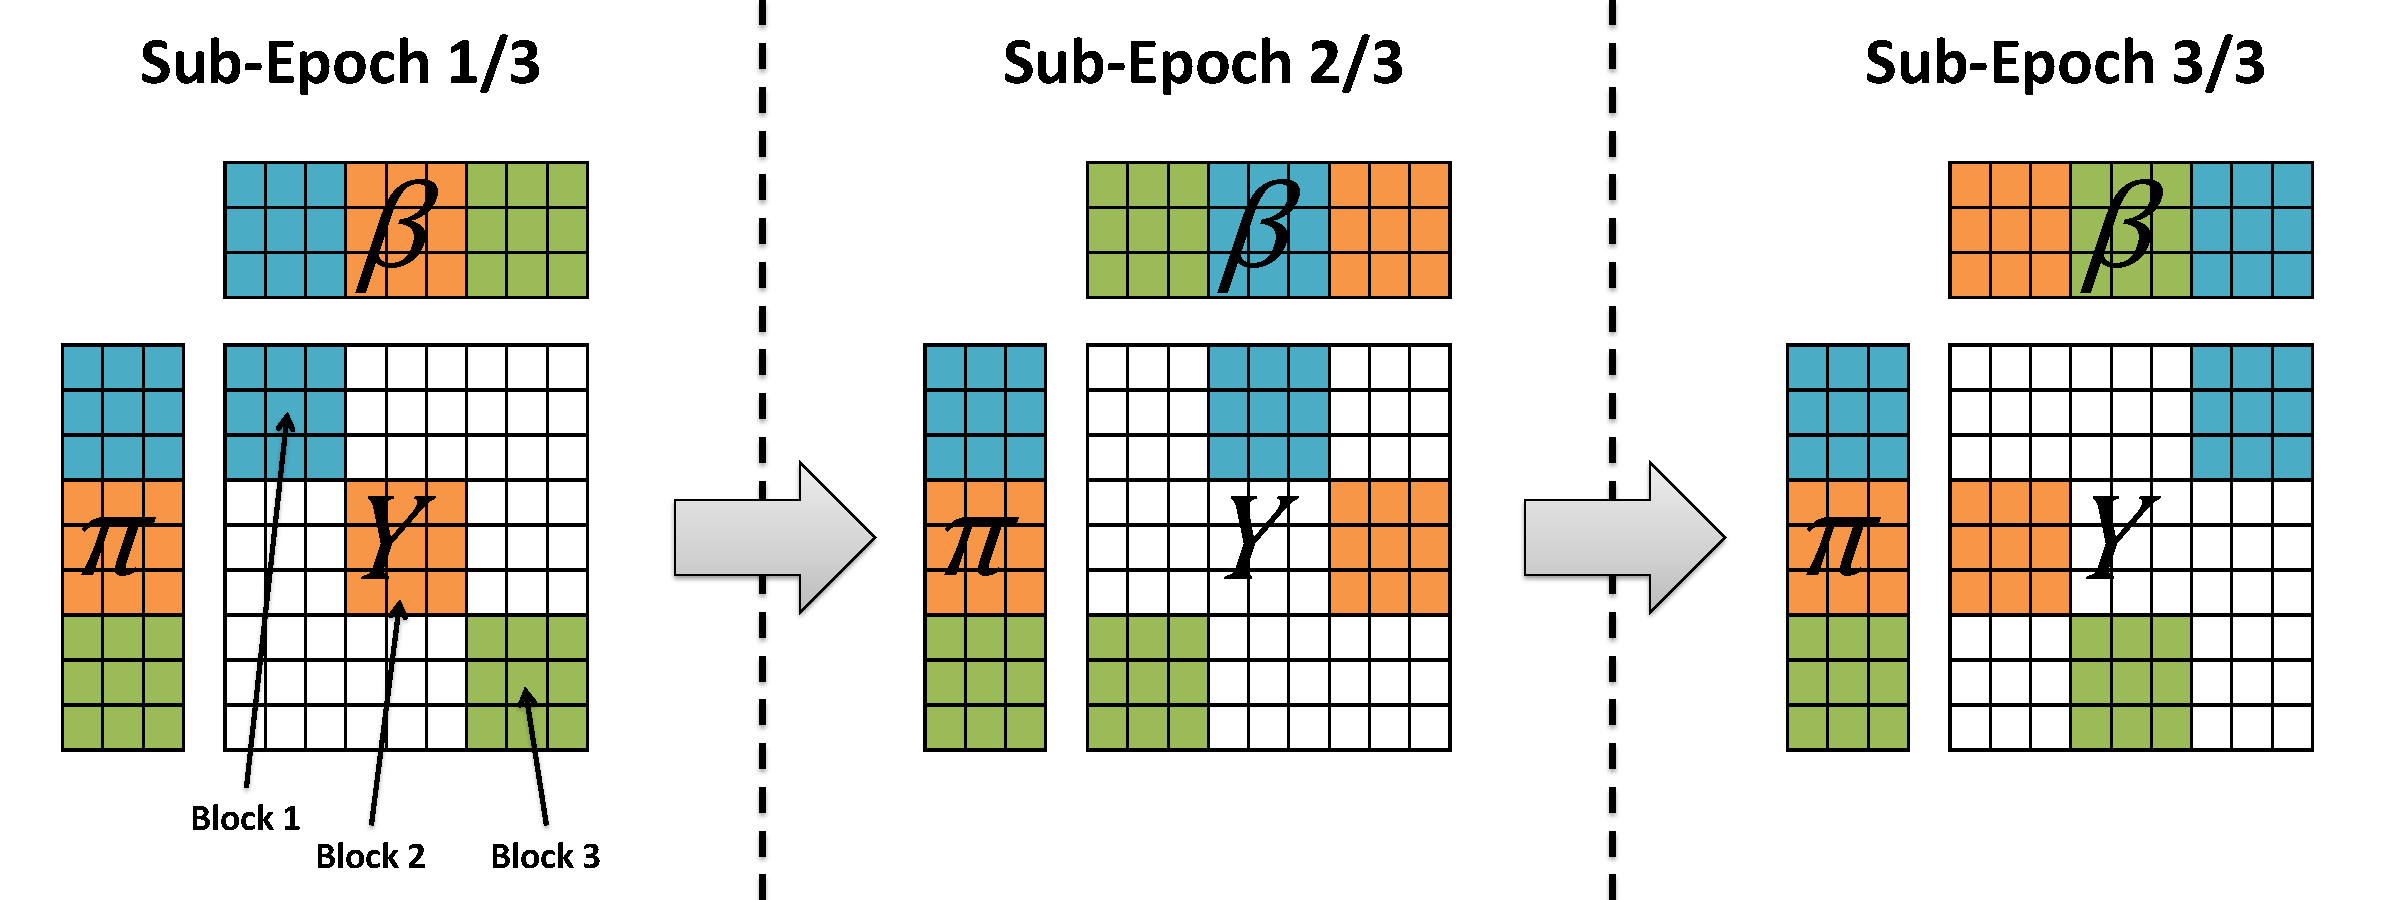
\includegraphics[width=\textwidth]{fig/partition.pdf}
\vspace{-0.6cm}
\caption{\small Partitioning strategy for data $Y$, model variables $\pi$, and parameters $\beta$.
We show one epoch broken into multiple sub-epochs (3 in this case).
Each sub-epoch is further divided into (colored) blocks, such that the data $Y_{i,j}$ (with its
associated variables $\pi_{i,\cdot}$ and parameters $\beta_{\cdot,j}$) from one block do not
share rows/columns with data $Y_{a,b}$ from another block. Taken together, all blocks from
all sub-epochs cover every element of $Y,\pi,\beta$.
}
\vspace{-0.4cm}
\label{fig:para-div}
\end{figure*}

\paragraph{High-level overview.}
To learn latent space models effectively on a distributed cluster,
we must exploit the interdependence of parameters and variables.
As a running example, consider the topic modeling objective $L(Y,\pi,\beta)$:
we can divide the data matrix $Y$ into a sequence of sub-epochs, where
each epoch consists of blocks that do not overlap on parameters $\beta$ and variables $\pi$,
and where the union over all epochs covers the entire matrix (Figure~\ref{fig:para-div}).
This blocking strategy is attributed to Gemulla {\it et al.}~\cite{Gemulla:2011:LMF:2020408.2020426}, and it
permits multiple machines to perform stochastic gradient descent (SGD) on different blocks in parallel,
on a Hadoop cluster. However, it requires all workers to process a roughly equal number of data-points
per block, which leads to problems with slow workers. In this paper, we intend to address this limitation. 
Our proposed algorithm allows faster workers to process extra data-points in their assigned block, which maximizes the cluster's computational efficiency. 
%and our algorithm and theoretical analysis removes this limitation, allowing faster workers to process extra datapoints in their assigned block, which maximizes the cluster's computational efficiency.

At a high level, our algorithm proceeds one epoch at a time, performing SGD on all blocks within an epoch in parallel. In order to satisfy the problem constraints, we must interleave projection steps with the SGD algorithm. In this respect, the parameters $\beta$ and variables $\pi$ must be handled differently: while the simplexial projection for variables $\pi$ can be performed by each worker independently of others, the simplexial projection for the parameters $\beta$ requires workers to repeatedly synchronize with each other. This cannot be done through the standard MapReduce programming model, so our Hadoop implementation deviates from the MapReduce scheme and allows workers to write to the Hadoop Distributed File System (HDFS) in order to communicate projection information with each other. We find that this scheme works well in practice, while dedicated, memory-based synchronization systems such as parameter servers~\cite{cipar2013solving,ahmed2012scalable,power2010piccolo} have the potential to perform even better.

\vspace{-0.2cm}
\paragraph{Partitioning strategy.}
More formally, let $\bold{\Psi}$ collectively refer to the variables and parameters
$\mathbf{\pi, \beta}$, and let $\psi$ refer to individual elements of $\bold{\Psi}$.
These definitions will make the subsequent analysis easier to understand.
Thus, we rewrite the topic modeling objective $L$ as: 
\begin{align}
\psi^{(t+1)}&= \psi^{(t)} - \eta_t \nabla
\loss_{Y_{i,j}}(\psi^{(t)}),
\label{equ:sgd-update-lda}
\end{align}
and we apply parameter/variable projections each time we execute Eq.~(\ref{equ:sgd-update-lda}).
Assuming the $\ell_2$ norm, the differential of $\psi$ with respect
to $\pi$ at a single data point $Y_{i,j}$ is
{\scriptsize
\begin{align}
	(\nabla L_{Y_{i,j}}(\psi))_\sigma &= 
	\left\{
	\begin{array}{ll}
		-2(Y_{i,j}-\sum_k \pi_{i,k}\beta_{k,j}
		)\beta_{\ell,j}  & \mbox{if } \sigma = \pi_{i,\ell} \\
		0 & \mbox{if } \sigma = \pi_{i',\ell},\ i\neq i'\\
	\end{array}
	\label{eqn:diff-lda}
\right.
\end{align}}
where $\sigma$ is the element of $\pi$ being differentiated, and $(\nabla L_{Y_{i,j}}(\psi))_\sigma = \frac{\partial L_{Y_{i,j}}}{\partial \sigma}$.
The differentials with respect to $\sigma = \beta_{j,\ell}$
are similar.
From these equations, we observe that the SGD update for $\pi_{i,\ell}$ at a particular datapoint
$Y_{i,j}$ depends only on a small subset of the variables and parameters: specifically,
$\pi_{i,k}, \beta_{k,j}$ where $k\in {1,\ldots,K}$ and $K$ is the number of topics we chose.
Notice that the $\pi$ all come from the same row $i$ as $Y_{i,j}$, while the $\beta$ all come
from the same column $j$.
Furthermore, the SGD updates for $\pi_{i,\ell}$ are zero for any datapoint $Y_{a,b}$ where $a \ne i$.
A similar observation holds for the parameters: the SGD update for $\beta_{r,j}$ is zero for
any datapoint $Y_{a,b}$ where $b\ne j$.

These observations lead to the following key insight: we can perform SGD on two datapoints $Y_{i,j}$ and $Y_{a,b}$ at the same
time, provided $i \ne a$ and $j \ne b$ --- in other words, as long as the datapoints do not
overlap on their rows or columns. An intuitive proof goes like this: SGD updates on $Y_{i,j}$ only touch the variable row $\pi_{i,\cdot}$
and the parameter column $\beta_{\cdot,j}$, and both of them do not overlap with $Y_{a,b}$'s variable row $\pi_{a,\cdot}$ and
parameter column $\beta_{\cdot,b}$. In other words, the SGD updates on $Y_{i,j}$ and $Y_{a,b}$
touch disjoint sets of variables $\pi$ and parameters $\beta$.
Furthermore, each $\pi_{i,\cdot}$ in row $i$ only ever depends on other $\pi$ in the same row $i$,
and similarly for $\beta_{\cdot,j}$ and other $\beta$ in column $j$. We therefore conclude that
all quantities associated with row $i$ and column $j$, namely $Y_{ij},\pi_{i\cdot},\beta_{\cdot j}$, are completely
independent of the quantities from row $a$ and column $b$, namely $Y_{ab},\pi_{a\cdot},\beta_{\cdot b}$.
Hence, datapoints with disjoint rows and columns can be simultaneously used for SGD updates~\cite{Gemulla:2011:LMF:2020408.2020426}.

From the perspective of data, model and parameter partitioning, we have essentially partitioned datapoints
$Y$, model variables $\pi$ and parameters $\beta$ into independent ``collections" $\mathcal{C}_{ij}$,
%\eric{do we have a better notation for collection? $(x,x)$ usually denotes a pair.}
where
$i$ is a row index and $j$ is a column index. In other words, the collection $\mathcal{C}_{ij}$ contains $Y_{ij},\pi_{i\cdot},\beta_{\cdot j}$,
and can be ``processed" (meaning that we run SGD on $Y_{ij}$ to update $\pi_{i\cdot}$ and $\beta_{\cdot j}$)
in parallel with any other collection $\mathcal{C}_{ab}$ where $a\ne i$, $b \ne j$.

We note that the above scheme applies to Dictionary Learning with only slight modification. For Mixed-Membership
Network Decomposition, the presence of the symmetric term $\theta B\theta^T$ presents additional challenges.
Instead, we replace $\theta B\theta^\top$ with $\theta C$ where $C := B\theta^\top$, and recover $B$ post-optimization
via pseudoinversion: $B = C\theta(\theta^\top \theta)^{-1}$. The inversion cost is reasonable since $\theta^\top \theta$ is $K\times K$,
while $K$ is rarely $\ge 1000$ in practice.

\vspace{-0.2cm}
\paragraph{Distributed update scheduling.}
Since collections $\mathcal{C}_{ij}$ with disjoint rows/columns can be processed
simultaneously, let us consider grouping
them into multiple blocks $S_b \subseteq Y$, such that the blocks have disjoint rows/columns (Figure~\ref{fig:para-div}).
While we cannot process collections $\mathcal{C}_{ij}$
within the same block in parallel (because they might share rows/columns), we can process collections from
{\it different} blocks in parallel, as they are guaranteed to be non-overlapping. Thus, if we managed to
construct $P$ non-overlapping blocks, we can spawn $P$ workers to perform SGD in parallel. Although it
is impossible to find a set of non-overlapping blocks that covers all of $Y$, we can find multiple disjoint sets of
non-overlapping blocks that, taken together, cover $Y$ completely (Figure~\ref{fig:para-div}). We call
these sets {\it sub-epochs}, which are processed sequentially (while the blocks within a sub-epoch
are processed in parallel). An {\it epoch} is a sequence of sub-epochs that fully covers $Y$.

%\eric{better directly use the name of the algorithm}
\ourmethod~differs from Gemulla~{\it et al.} in that
within a sub-epoch, we allow different worker-blocks to perform varying numbers of SGD updates per collection $\mathcal{C}_{ij}$
(whereas Gemulla~{\it et al.} require equal numbers of updates per worker).
This makes our algorithm much more efficient whenever there are slow
worker machines (which are common in large clusters),
since faster workers can keep running until synchronization, rather than
wasting computational time waiting for slower workers to catch up. The full algorithm is shown in Algorithm \ref{algo:lda},
and we shall prove that it converges, along with several other important properties.

\IncMargin{1em}
\begin{algorithm}[t]
\small
\SetAlgoLined
Input : $Y,\beta, \pi$,~sub-epoch~size~$d$\\
$\pi\leftarrow \pi_0$, $\beta\leftarrow \beta_0$\\
Block $Y,\pi,\beta$ into corresponding $w$ blocks\\
\While{not converged}{
Pick step size $\eta_S$\\
		Pick $w$ blocks($S_{1},...,S_{w}$) to form sub-epoch $S$\\
		\For{$b=0,\ldots,w-1$ \textbf{in parallel}}{
			Run SGD on the training points $Y_{ij}\in S_{b}$\\
			// (until every block is ready to synchronize)\\
			// Each worker-block $S_{b}$ can touch datapoints\\
			// multiple times if other blocks are slow.\\
			Apply appropriate projections\\
			// (e.g. on variables $\pi$ in topic modeling)\\
		}
		Apply appropriate projections\\
		// (e.g. on parameters $\beta$ in topic modeling)\\
}
\caption{\small \ourmethod, our slow-worker agnostic learning algorithm, applied to topic modeling.}
\label{algo:lda}
\end{algorithm}

\vspace{-0.3cm}
\section{Theoretical Analysis}
\vspace{-0.2cm}

We now analyse \ourmethod~(Algorithm~\ref{algo:lda}), and prove
that our strategy of allowing multiple SGD iterations on each data/variable/parameter
collection $\mathcal{C}_{ij} = \{Y_{ij},\pi_{i\cdot},\beta_{\cdot j}\}$
leads to faster convergence (under reasonable conditions). Furthermore, we analyze the variance of
the model state $\Psi$ under \ourmethod, and show that it remains bounded under certain assumptions.
Briefly, the variance can be attributed to two aspects of our partitioning strategy: (1) running
multiple blocks within a sub-epoch in parallel, and (2) splitting
the data matrix into a sequence of sub-epochs. These variance bounds
distinguish our analysis from Gemulla {\it et al.}~\cite{Gemulla:2011:LMF:2020408.2020426}, who did not provide
such bounds for their blocking strategy.
We will show that allowing additional iterations on fast workers
is better than waiting for slow workers, by
proving that the model state $\Psi$'s variance converges to zero under an appropriate step-size sequence.

Assume we have $w$ worker processors, and that in each sub-epoch, every processor
is assigned to a distinct block $i$ --- henceforth, we shall use index $i$ to
refer interchangeably to processors or blocks. We now define the following terms:
\vspace{-0.2cm}
\begin{definition}
{\rm :} {\bf Key states and parameters}
\end{definition}
\vspace{-0.5cm}
{\small
\begin{itemize}
    \setlength{\itemsep}{0.6pt}
    \setlength{\parskip}{1pt}
\item $n_i$, $\kappa_i$ and $N_w$: Let $n_i$ be the number of datapoints
that worker $i$ touches (with repetition) in its assigned block, before
transitioning to the next sub-epoch. In other words, if worker $i$ was assigned $n$
datapoints, and touches each point $\kappa_i \geq 1$ times on average, then\\[-0.5cm]
\begin{align}
n_i = \kappa_i n \qquad \text{and} \qquad N_w = \sum_{i=1}^w n_i 
\label{eqn:workerIpoints}
\end{align}\\[-0.7cm]
  \item $\eta_t$: SGD step size at iteration $t$. An iteration is defined as one
SGD update on one datapoint.
  \item $ \nabla\mathcal{L}(\itert{\psi})$: Exact gradient at iteration
$t$.
  \item $\delta \itert{L}(\itert{V},\itert{\psi})$: Stochastic gradient at
  iteration $t$, i.e. $\nabla \loss_{Y_{i,j}}(\psi^{(t)})$ for some $i,j$.
  \item  $\varepsilon_t$: Error due to stochastic update at iteration $t$, $\left[
\nabla\mathcal{L}(\itert{\psi}) - \delta
\itert{L}(\itert{V},\itert{\psi})\right]$.
  \item $\atiter{\psi}{t}$ : Model state $\psi$ (see
  Eq.~\ref{equ:sgd-update-lda}) at iteration $t$.\\[-0.6cm]
\end{itemize}
}

We now introduce
$\atiter{V}{t}(\atiter{\psi}{t+1},\atiter{\psi}{t})$, a state potential
function defined over a previous state $\atiter{\psi}{t}$, a future state
$\atiter{\psi}{t+1}$, and the data points $\atiter{y}{t}$ picked at
iteration $t$.

\vspace{-0.2cm}
\begin{definition}
{\rm :} {\bf State Potential Function ($V$)} 
\end{definition}
\vspace{-0.2cm}

$V^{(t)}$ encodes the probability
that $\atiter{\psi}{t}$ will be updated to $\atiter{\psi}{t+1}$ when the algorithm
performs the stochastic update over datapoint $y^{(t)}$. We also define an $n_i$-dimensional
state potential $V = \left(\atiter{V}{t+1}, \atiter{V}{t+2}\ldots \atiter{V}{t+n_i} \right)$,
which encodes the probability distribution of updates caused by all $n_i$ iterations in block $i$ of
a sub-epoch (assuming that block $i$ starts at iteration $t+1$).

Next, assumptions on the error terms $\varepsilon_t$ and step sizes $\eta_i$:
\vspace{-0.2cm}
\begin{assumption}
{\rm:} {\bf Errors and Step-sizes}
\end{assumption}
\vspace{-0.4cm}
{\small
\begin{itemize}
    \setlength{\itemsep}{0.6pt}
    \setlength{\parskip}{1pt}
  \item \textbf{Martingale difference error $\varepsilon_t$}:
  The error terms $\varepsilon_t$ form a martingale difference sequence. 
  \item \textbf{Variance bound on $\varepsilon_t$}:
  For all $t$, we have $E[\varepsilon_t^2]<D$.
  \item \textbf{Step size $\eta_t$ assumption}: $\sum\eta_t^2 <\infty$.\\[-0.6cm]
\end{itemize}}
The condition that error terms are a martingale
difference sequence is weaker (easier to satisfy) than assuming error terms
$\varepsilon_t$ are independent of each other. The martingale difference
assumption means that the stochastic gradient $\delta \itert{L}(\itert{V},\itert{\psi})$,
when conditioned on the initial model state $\psi^{(0)}$ and previous gradients $\delta
\iiter{L}(\iiter{V},\iiter{\psi})$ for all $i<t$, depends only on the current model
stae $\itert{\psi}$. \ourmethod~satisfies this martingale assumption because
our blocking strategy ensures that parallel parameter updates (from different blocks)
never overlap on the same elements of $\psi$. For models with more complex
dependency structures (e.g. arbitrary graphical models), the martingale assumption may
allow for parallelization opportunities even when such non-overlapping structure is absent.

\vspace{-0.2cm}
\subsection{Convergence of \ourmethod}
\vspace{-0.1cm}
First, using the definition of $V^t$, we obtain the relation
{\small
\begin{equation}
p(\atiter{\psi}{t+1}|\atiter{\psi}{t}) d\atiter{\psi}{t} =
p(V^{(t)}(\atiter{\psi}{t+1},\atiter{\psi}{t}))
dV^{(t)}(\atiter{\psi}{t+1},\atiter{\psi}{t}).
\label{eqn:potentialDef}
\end{equation}}
We can interpret this equation as follows:
fix an particular update event
$\atiter{\psi}{t} \rightarrow \atiter{\psi}{t+1}$, then
$V^{(t)}(\atiter{\psi}{t+1},\atiter{\psi}{t})$
represents the event that some datapoint $\atiter{y}{t}$ gets chosen,
while $dV^{(t)}(\atiter{\psi}{t+1},\atiter{\psi}{t})$ is the
probability that said choice leads to the update event $\atiter{\psi}{t} \rightarrow \atiter{\psi}{t+1}$.
The intuition here is that $\itert{V}=\itert{V}(\itertO{\psi},\itert{\psi})$ is a 
function that keeps track of the state of $\itert{\psi}$ and $\itertO{\psi}$,
and that depends on the datapoint $\itert{Y_{i,j}}$ chosen by the SGD update.

Next, by definition of a martingale difference sequence:
\begin{eqnarray}
E\left[\nabla\mathcal{L}(\itert{\psi}) - \delta
\itert{L}(\itert{V},\itert{\psi}) \;\vert\; \right. \qquad &&\nonumber \\
\left. \delta
\iiter{L}(\iiter{V},\iiter{\psi}),\iiter{\psi},i<t,\itert{\psi}\right] &=&
0, \nonumber \\
E\left[\varepsilon_t|\varepsilon_i,i<t\right] &=& 0.
\label{eqn:martingaleAssumption}
\end{eqnarray}
In other words, the error term $\varepsilon_t$ has zero expectation when
conditioned on previous errors.
We now have the necessary tools to provide a convergence guarantee:
\vspace{-0.2cm}
\begin{theorem}
	The stochastic updates 
	$\psi^{(t+1)}= \psi^{(t)} - \eta_t \nabla \loss_{Y_{i,j}}(\psi^{(t)})$ as
	described in algorithm~\ref{algo:lda} and the exact updates
	$\psi^{(t+1)}=\itert{\psi} - \eta_t\nabla \mathcal{L}(\itert{\psi})$ (for
	an exact gradient descent) converge to the same set of limit points
	asymptotically, given that the error terms $\varepsilon_t$ are a martingale
	difference sequence, and $E[\varepsilon_i^2]<D$ (bounded variance), and
	$\sum\eta_i^2 <\infty$.
	\label{theo:asymptotConverge}
\end{theorem}
We defer the proof to the appendix.
The above theorem says that, asymptotically, the error terms cancel each other out,
and therefore our stochastic algorithm will find the same set of optima as an
exact gradient aglrotihm.

\vspace{-0.2cm}
\subsection{Variance of $\psi$ within a sub-epoch}
\vspace{-0.1cm}
We now bound the variance of the model state $\psi$, when
it is updated inside block $i$ in a sub-epoch.
\vspace{-0.2cm}
%\eric{be consistent about whether you use normal font or italic for assumption or definition etc.}
\begin{assumption}
{\rm Assume for simplicity that the parameter being updated in block $i$ is univariate. 
The analysis can be easily extended to multivariate updates.}
\end{assumption}
\vspace{-0.2cm}
\begin{theorem}
\label{thm:psi_variance_within_subepoch}
Within block $i$, suppose we update the model state $\psi$ using $n_i$ datapoints (Eq.~\ref{eqn:workerIpoints}).
Then the variance of $\psi$ after those $n_i$ updates is
\begin{align*}
Var(\raisePsi{t+n_i}) =& Var(\psi^t)- 2\eta_tn_i\Omega_0(Var(\psi^t)) \nonumber\\
&-2\eta_tn_i\Omega_0CoVar(\psi_t,\bar{\delta_t}) + \eta_t^2n_i\Omega_1 \nonumber\\ 
&+ \underbrace{\order{\eta_t^2\rho_t} +
\order{\eta_t\rho_t^2} +
\order{\eta_t^3}+ \order{\eta_t^2\rho_t^2}}_{\Delta_t}
\end{align*}
Constants $\Omega_0$ and $\Omega_1$ are defined in
Theorems 1 and 2 in 
the Appendix.
\end{theorem}
The proof is left to the Appendix.
Note that the constants $\Omega_0$ and $\Omega_1$ are independent of the datapoints picked or
the iteration number; they only depend on the global optima of the problem.
The above theorem consists of 4 important terms on the first line, plus another 4 cubic (or higher order)
terms $\Delta_t$ that quickly converge to zero and can be ignored. The basic intuition is as follows:
when the algorithm is far from an optimum, $Var(\atiter{\psi}{t})$ and $CoVar(\atiter{\psi}{t},\bar{\delta}_t)$
are large, so the 2nd and 3rd terms dominate and the variance of $\psi$ decreases quickly. When
close to an optimum, the constant 4th term with $\Omega_1$ dominates, causing the algorithm
to oscillate unless the step size $\eta^2_t$ is small --- which we have ensured via shrinking step sizes $\sum \eta^2_t < \infty$.
Hence, the 4th term also shrinks to zero as $t \rightarrow \infty$, and therefore the variance of $\psi$
also decreases when close to an optimum.

\vspace{-0.2cm}
\subsection{Variance of $\psi$ between sub-epochs}
\vspace{-0.1cm}
Let us consider the variance of $\psi$ across entire sub-epochs. First, note that within
a sub-epoch, two blocks $Z_i$ and $Z_{i^\prime}$ are independent if for
each datapoint $y \in Z_i$ and $y^{'} \in Z_{i^\prime}$, the following holds:
\begin{align}
\nabla L_{y}(\psi) = \nabla L_{y}(\psi -
\eta \nabla L_{y_{'}}(\psi)) \nonumber\\ 
{\rm and}\quad \nabla L_{y_{'}}(\psi) =
\nabla L_{y_{'}}(\psi - \eta \nabla L_{y}(\psi))
\label{eqn:blockIndependence}
\end{align}
In other words, even when the model state $\psi$ is perturbed by the stochastic gradient
on $y^\prime$, the stochastic gradient on $y$ must not change (and vice versa).
By our earlier argument on collections $\mathcal{C}_{ij} = \{ Y_{ij},\pi_{i\cdot},\beta_{\cdot j} \}$,
this condition holds true for any pair of points from distinct blocks.
Thus, within a sub-epoch, distinct blocks $Z_i$ and $Z_{i^\prime}$ operate
on disjoint subsets of $\Psi$, hence their update equations are independent of each other.
At the end of a sub-epoch $S_{n+1}$, the algorithm synchronizes the model state
$\Psi_{S_{n+1}}$ by aggregating the non-overlapping updates
$\delta\psi^i_{S_{n+1}}$ from all blocks $S^i_{n+1}$. Therefore, we can write the variance
$Var(\Psi_{S_{n+1}})$ at the end of sub-epoch $S_{n+1}$ as
{\scriptsize
\begin{align}
&Var(\Psi_{S_{n+1}}) = \sum_{i=1}^{w}Var(\psi^i_{S_{n+1}}) \label{eqn:interVar} \\
=& \sum_{i=1}^{w}\bigg[Var(\psi^i_{S_{n}})  -
2\eta_{S_n}n_i\Omega_0^i(Var(\psi^i_{S_{n}})) \nonumber\\
&-2\eta_{S_n}n_i\Omega_0^i(CoVar(\psi^i_{S_{n}},\bar{\delta}_{S_n}^i))
+ \eta_{S_n}^2n_i\Omega_1^i + \Delta_{S^i_{n}}\bigg] \nonumber \\
=& Var(\Psi_{S_{n}}) -
2\eta_{S_n}\sum_{i=1}^{w}n_i\Omega_0^iVar(\psi^i_{S_{n}}) \nonumber \\
&-2\eta_{S_n}\sum_{i=1}^{w}n_i\Omega_0^iCoVar(\psi^i_{S_{n}}
,\bar{\delta}_{S_n}^i)
+ \eta_{S_n}^2\sum_{i=1}^{w}n_i\Omega_1^i + \order{\Delta_{S_{n}}},
\nonumber
\end{align}}
where the 2nd line is proven in the Appendix.
The interpretation is similar to
Theorem \ref{thm:psi_variance_within_subepoch}: when far from an optimum,
the negative terms dominate and the variance shrinks; when close to an optimum,
the positive $\Omega_1^i$ term dominates but is also shrinking because of the step sizes $\eta^2_{S_n}$.
Again, we can ignore the higher-order terms $\order{\Delta_{S_{n}}}$.

\vspace{-0.2cm}
\subsection{Slow-worker agnosticism}
\vspace{-0.1cm}
We now explain why allowing fast processors to do extra updates is beneficial.
In Eq.~\ref{eqn:interVar}, we saw that the variance after each sub-epoch $S$ 
depends on the number of datapoints touched $n_i$ and the step size $\eta_{S_n}$.
Let us choose $\eta_{S_{n}}$ small enough so that the variance-decreasing terms dominate, i.e.
{\small
\begin{align}
&2\eta_{S_n}\sum_{i=1}^{w}n_i\Omega_0^iVar(\psi^i_{S_{n}}) +
2\eta_{S_n}\sum_{i=1}^{w}n_i\Omega_0^iCoVar(\psi^i_{S_{n}},\bar{\delta}_{S_n}^i) \nonumber \\
&\quad> \eta_{S_n}^2\sum_{i=1}^{w}n_i\Omega_1^{i}.
\label{eqn:varianceDecreaseCondition}
\end{align}}
This implies $Var(\Psi_{S_{n+1}}) < Var(\Psi_{S_{n}})$.
Hence, using more datapoints $n_i$ decreases the variance of the model state $\psi$,
provided that we choose $\eta_{S_n}$ so that Eq.~\ref{eqn:varianceDecreaseCondition} holds.
This is easy to satisfy: the RHS of Eq.~\ref{eqn:varianceDecreaseCondition} is $\order{\eta_{S_n}^2}$
while the LHS is $\order{\eta_{S_n}}$, so we just set $\eta_{S_n}$ small enough.

Let us now take stock:
Eq.~\ref{eqn:varianceDecreaseCondition} tells us that using additional datapoints
in any block can decrease the variance of $\Psi$, while Theorem~\ref{theo:asymptotConverge}
tells us that the algorithm converges asymptotically, regardless of the number of processors
and the number of datapoints assigned to each processor.
Because the algorithm converges, decreasing the variance will only move $\Psi$ towards an optimum,
and therefore it makes sense for faster processors to perform more updates
(with appropriate choice of step size $\eta_{S_n}$) and decrease the variance of $\Psi$,
rather than wait for slow processors to finish.
However, if the step size $\eta_{S_n}$ is set incorrectly, then using
too many updates $n_i$ could increase the variance of $\Psi$.

%\eric{This is a bit surprising and counter-intuitive: why not in such case just go totally async? or it suggest that async actually is guaranteed to converge, but just with a slower rate? How SSP would help?}
It is important to note that \ourmethod~is {\it not} equivalent to fully
asynchronous computation (e.g. Hogwild~\cite{niu2011hogwild}), in which every worker
can proceed to arbitrary data points, variables and parameters, without regard to what
other workers are doing. \ourmethod~requires that all workers advance to the next sub-epoch
at the same time, in order to preserve independence between parallel blocks (and thus the
martingale condition). Bounded-synchronization schemes like Stale Synchronous Parallel~\cite{ho2013more,cipar2013solving}
may allow \ourmethod~to advance workers to different sub-epochs at different times,
thus increasing the effectiveness of fast workers without losing of convergence guarantees.
 
\vspace{-0.3cm}
\section{Experiments}
\vspace{-0.2cm}


\begin{figure*}[t]
\vspace{-0.4cm}
\centering
\begin{tabular}{|c|c|c|c|}
\hline
\multicolumn{4}{|c|}{\bf Topic Modeling} \\
\hline
Convergence Plots & \# of Topics & \# of Processors & \# of Docs \\
\hline
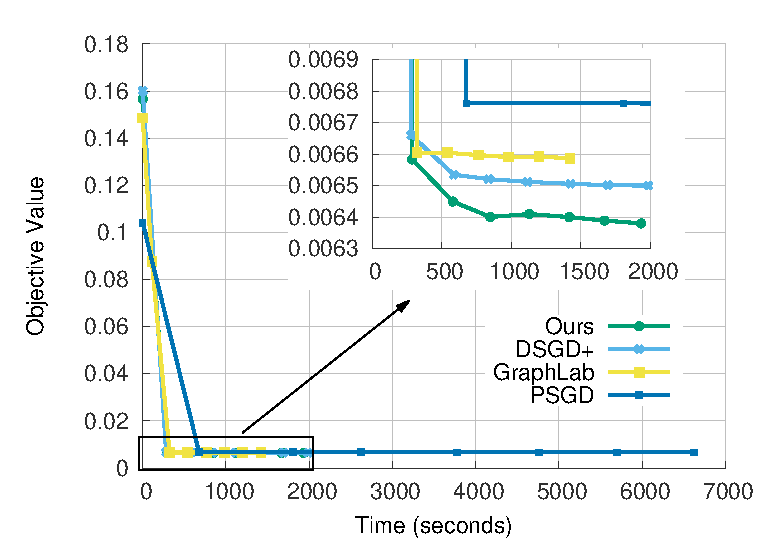
\includegraphics[width=0.23\textwidth]{fig2/lda_convergence.eps} &
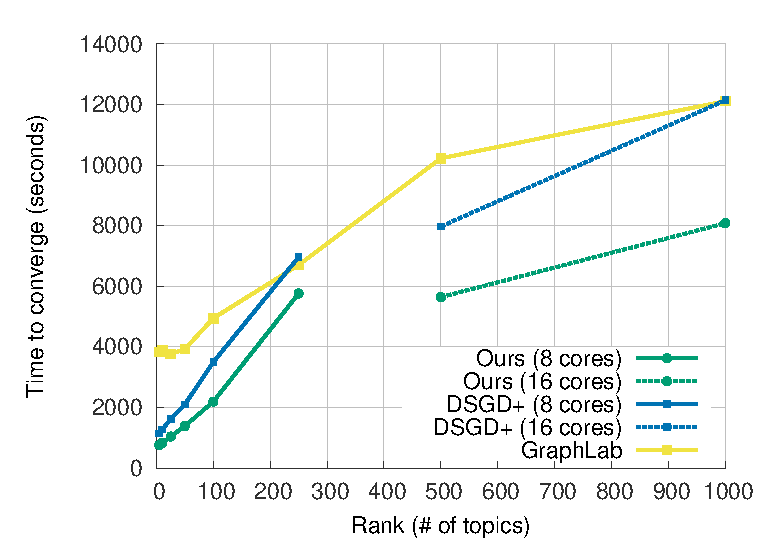
\includegraphics[width=0.23\textwidth]{fig2/lda_rank.eps} &
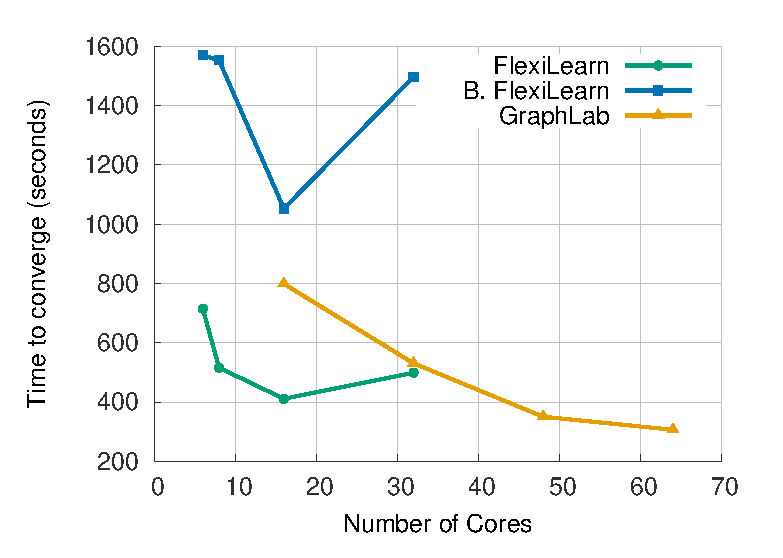
\includegraphics[width=0.23\textwidth]{fig2/lda_machines.eps} &
\includegraphics[width=0.23\textwidth]{fig2/lda_datasize.eps} \\
\hline
{\bf Topic Modeling} & {\bf Dictionary Learning} & \multicolumn{2}{|c|}{\bf Mixed Membership Network Decomposition} \\
\hline
Machines Required & Convergence Plots & \multicolumn{2}{|c|}{Convergence Plots} \\
\hline
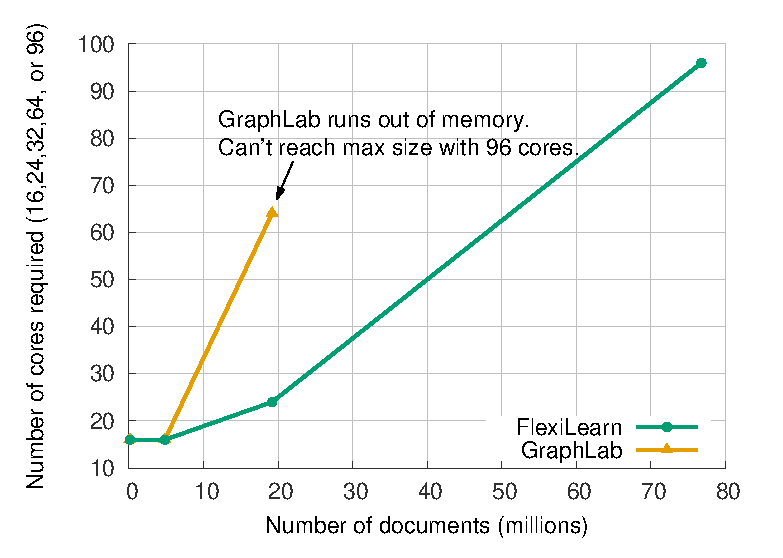
\includegraphics[width=0.23\textwidth]{fig2/lda_machines_failing.eps}
& 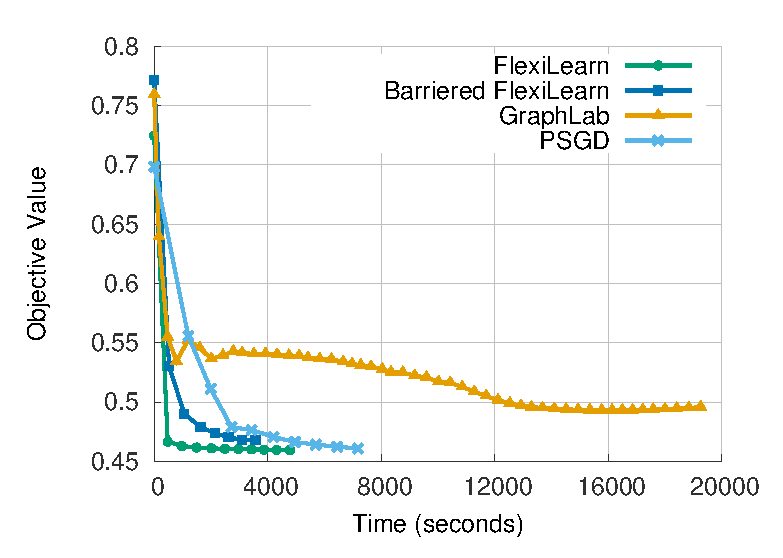
\includegraphics[width=0.23\textwidth]{fig2/dict_convergence.eps}
& \multicolumn{2}{|c|}{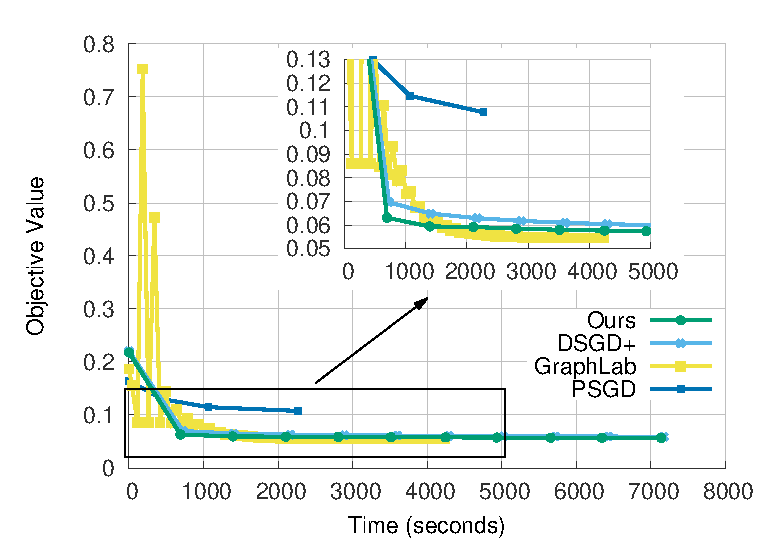
\includegraphics[width=0.23\textwidth]{fig2/mmsb_convergence.eps}} \\
\hline
\end{tabular}
\vspace{-0.3cm}
\caption{\small Convergence and scalability plots for the three models (topic modeling, dictionary learning, mixed-membership
network decomposition), under our \ourmethod{} and baselines (DSGD, PSGD, GraphLab). Unless otherwise stated in the plot, all methods were run with 16 cores
and rank $K=25$. For all topic modeling plots except ``\# of Docs" and ``Machines Required", we used the NyTimes4 dataset (Table \ref{tab:dataset}).
The convergence plots reveal the objective trajectory and final value of each method,
while the scalability plots show how each method fares (on topic modeling) as we increase the problem rank, number of processor cores, and data size.
In the bottom left, we also show the minimum number of machines required for a given topic modeling dataset size, for
\ourmethod{} and GraphLab.}
\vspace{-0.5cm}
\label{fig:results}
\end{figure*}

We compare our slow-worker agnostic algorithm implemented on Hadoop
to three self-implemented baselines: (a) Distributed SGD~\cite{Gemulla:2011:LMF:2020408.2020426}
on Hadoop, (b) Parallel SGD~\cite{zinkevich2010parallelized} on Hadoop,
and (c) constrained Matrix Factorization on distributed GraphLab~\cite{low2012distributed}, a
modification of the default GraphLab MF toolkit that regularly projects variables to maintain constraints
(without altering the input graph). We test all 4 methods
on our 3 latent space models: topic modeling, dictionary learning, and mixed-membership network decomposition.
We also tune all methods to their optimum parameters, before taking results.

Compared to the baselines, our method has several theoretical and practical advantages: unlike DSGD, our algorithm allows fast workers
to continue doing work while waiting for slow workers to synchronize, and unlike PSGD, we explicitly partition the
data/variables/parameters into collections $\mathcal{C}_{ij} = \{Y_{ij},\pi_{i\cdot},\beta_{\cdot j}\}$ instead of averaging updates
over all data points. Finally, we note that GraphLab is poorly-suited for implementing the simplex and inner-product constraints
required by our topic modeling, dictionary learning and mixed-membership network decomposition models. This is because
the constraints are over entire matrix rows, creating dependencies over all row variables --- which is
especially problematic for topic modeling, because the vocabulary matrix $\beta$ has $V$ columns, and
$V$ can be $\ge 100K$ words in practice. As we shall show, such long-range dependencies hurt GraphLab's
performance, because GraphLab picks sets of variables for updating without regard to the constraints --- whereas
a better strategy is to schedule as many dependent elements together as possible.

\vspace{-0.2cm}
\paragraph{Cluster Hardware}
%DO NOT REVEAL ANY INFORMATION THAT SUGGESTS WE ARE FROM CMU
The Hadoop algorithms (ours, DSGD, PSGD) were run on a Hadoop cluster
with the following machine specifications: 2x Intel Xeon E5440 @ 2.83GHz (8 cores per machine),
16GB RAM, 10Gbit Ethernet.
Because the Hadoop cluster did not support MPI programs, we ran GraphLab on a
newer cluster with the following machine specifications: 2x Intel Xeon E5-2450 @ 2.1-2.9GHz
(16 cores per machine), 128GB RAM, 10Gbit Ethernet. Thus, the GraphLab experiments
have significantly more memory, but slightly slower processors.
%As we shall see, our method significantly outperforms
%GraphLab, even when the latter is given far more processor cores (in addition to much
%more RAM and a much faster network interface).

\vspace{-0.2cm}
\paragraph{Datasets}
Statistics for all datasets are summarized in Table~\ref{tab:dataset}.
For topic modeling, we simulated datasets of various sizes, using the 300K-document
NY Times dataset as a building block. The resulting $\beta$ matrices contain
102,660 columns (words), and between 1.2M to 76.8M rows (documents); zero word counts
are treated as missing entries.
For dictionary learning, we used a 630,716-image (rows) sample from ImageNet~\cite{imagenet_cvpr09},
with 1000 features per image (columns). The resulting matrix is fully dense (no missing entries).
For mixed-membership network decomposition, we used the Stanford web graph~\cite{Leskovec08communitystructure},
with 281,903 vertices (rows and columns). The resulting adjacency matrix contains all edges, as well as
$0.5\%$ of the non-edges (all other non-edges are treated as missing entries).

%For dictionary learning \abhi{we used a random half of the imagenet dataset~\cite{imagenet_cvpr09}. This dataset has only non-zeros entries and our algorithm treats not present entries as missing. Hence we added all the zero pixels to the data. The used data set has 630,716 images with each image a 1000 pixel vector. The size of the dataset after addition of zero pixels is 7.99 gbs.}... \qirong{todo}

%For mixed-membership network decomposition \abhi{The dataset is Stanford webgraph~\cite{Leskovec08communitystructure}. It has 281,903 vertices. MMSB models edges that are present as well as those that are absent. Due to this we subsample 0.5\% of the zero edges to infer the correct set of role-vectors. We can chose to not model all zero edges as long as we model a significant porportion of them~\cite{}. The modified dataset has 312,808,228 zero and non-zero edges and is 4.46 gbs huge.}... \qirong{todo}
%\abhi{Table~\ref{tab:dataset}}

\begin{table}
\vspace{-0.4cm}
\centering
\scriptsize
\begin{tabular}{c|c|c|c|} %\hline
{\bf Dataset} & {\bf Dimensions} & {\bf Nonzeros} & {\bf Size (GB)} \\ \hline\hline
\nytimes  & $0.3*10^6\times$102,660 & $0.1*10^9$ &  1.49  \\ \hline
%\pubmed & $8.2*10^6\times$141,043 &  $0.73*10^9$ & 11.19  \\ \hline
\imagenet & $0.63*10^6\times$1,000 & $0.63*10^9$ & 7.99  \\ \hline
%\twitter & $41.6*10^6\times 41.6*10^6$ & $1.5*10^9$ & 23.99 \\ \hline
\webgraph & $0.28*10^6\times 0.28*10^6$ & $0.31*10^9$ & 4.46 \\ \hline
\snytimes{4} & $1,2*10^6\times$102,660 & $0.4*10^9$ &  6.08  \\ \hline
\snytimes{16} & $4.8*10^6\times$102,660 & $1.6*10^9$ &  25.12  \\ \hline
\snytimes{64} & $19.2*10^6\times$102,660 & $6.4*10^9$ &  103.4  \\ \hline
\snytimes{256} & $76.8*10^6\times$102,660 & $25.6*10^9$ &  421.42  \\
\hline
\end{tabular}
\vspace{-0.2cm}
\caption{\small Dimension, size and nonzero statistics for our datasets.
Size is the file size in gigabytes. The biggest dataset (\snytimes{256}) is approximately 0.5
terabytes. Note that the \imagenet dataset is 100\% dense. }
\label{tab:dataset}
\vspace{-0.5cm}
\end{table}

\vspace{-0.2cm}
\paragraph{Stopping Criteria}
Unless otherwise stated, we stop each method when it has reached convergence, defined
as when its objective function does not change by more than $\pm 0.0005$ in successive iterations.

\vspace{-0.2cm}
\paragraph{Parameter Tuning}
...

\vspace{-0.2cm}
\paragraph{Results and Discussion}

\begin{table}
\centering
\small
\begin{tabular}{c|c|c|}
{\bf \ourmethod{} Model} & {\bf Wait/Sync Time} & {\bf Epoch Time} \\ \hline\hline
Dictionary Learning  & 32.6 & 471 \\ \hline
Topic Modeling & 110.6 & 391 \\ \hline
MM Network Decomp. &182 & 692 \\ \hline
\end{tabular}
\vspace{-0.2cm}
\caption{\small
Comparison of synchronization time vs epoch time,
for each ML model under \ourmethod{}. Dictionary learning has the smallest wait:epoch ratio,
because the input matrix is fully dense (hence every worker has the same workload). In contrast,
topic modeling has the highest wait:epoch ratio, because the normalization constraints on the topic-word matrix
impose additional synchronization costs. As a result, the fast workers in topic modeling get to perform many
more additional updates, and hence topic modeling converges in fewer iterations than dictionary learning.}
\label{tab:waitTime}
\vspace{-0.5cm}
\end{table}

Our results are shown and explained in Figure \ref{fig:results}. The convergence plots reveal that
our method converges faster and to a better solution than all three baselines, on all three ML models.
The scalability plots also reveal that our method converges faster (on topic modeling)
for any number of topics and documents, and generally requires fewer processors to converge quickly.
We note that GraphLab takes more than twice as long as \ourmethod{} to converge (noting
that the GraphLab machines had a slightly slower average clockspeed).
Moreover, GraphLab sometimes oscillates because its local
vertex synchronization prevents it from applying the global projections frequently enough.

The bottom left plot shows the minimum number of machines required by \ourmethod{} and GraphLab
for topic modeling on a given number of documents. Here, the primary reason for needing more machines is memory,
and we see that GraphLab requires additional machines at a faster rate (despite having 128GB per 16-core machine),
whereas \ourmethod{} scales much more gently (even with only 16GB per 8-core machine) --- this can
be explained by \ourmethod{}'s use of Hadoop and HDFS, so it does not have to load the entire model into memory
(unlike GraphLab).

%In terms of scalability, our method consistently maintains its lead as the problem rank (number of topics,
%dictionary bases, or network roles), number of processors used, or data size increases.
Compared to DSGD and PSGD, \ourmethod{} succeeds beacuse it (1) it partitions both data and model variables
to accounts for dependencies (which PSGD lacks), while (2) it allows faster workers
to do more work before synchronization (which DSGD lacks). In particular, PSGD's lack of partitioning
forces it to hold the entire model on each machine, which becomes a memory bottleneck for rank $K\ge 100$.
Moreover, PSGD makes one machine average all models at the end, which is a computational bottleneck ---
hence PSGD does not scale well with additional cores.

Table \ref{tab:waitTime} provides insights about slow and fast workers in \ourmethod. For example, dense
input matrices (e.g. our dictionary learning dataset) result in balanced workloads, thus every worker is equally
balanced. On the other hand, the topic-word matrix constraints in topic modeling
increase inter-epoch synchronization times, providng an opportunity for workers to conduct extra updates.

Although \ourmethod{} exhibits good performance, there remain areas for improvement.
We note that \ourmethod{} exhibits diminishing returns when going from 16 to 32 cores on topic modeling.
This is due to increased synchronization costs, which dominate the computational benefits from using additional cores.
We expect that moving from Hadoop to a parameter server system~\cite{ho2013more} will
alleviate the synchronization bottleneck, thus allowing \ourmethod{} to harness more machines.
Furthermore, while \ourmethod's row/column-wise partitioning strategy for data/variables/parameters
works well for the latent space models we have presented, it does not apply to all possible ML models:
for example, graphical models and deep networks can have arbitrary structure between parameters and variables,
while problems on time-series data will have sequential or autoregressive dependencies between datapoints.
In such cases, a row/column-wise partitioning will not work. Nevertheless, the {\it idea} and basic theoretical analysis of
grouping data, variables and parameters into independent collections still holds; only the partitioning
strategy needs to be changed. This opens up rich possibilities for future work on general-purpose partitioning algorithms
under our framework.

%Additionally, the relatively poor performance
%of GraphLab highlights the weakness of graph-based platforms at dealing with constrained optimization
%problems --- such graph platforms perform optimally when updating small, locally-connected sets of variables,
%but falter on models that contain many dependencies (e.g. normalization constraints over 100K variables).

%The convergence plots (left) reveal that, in addition to oscillating, GraphLab does not come close to the same
%solution quality (measured via the loss function) as our method and the other baselines.
%Even when GraphLab is given significantly more cores, it still fails to beat all other methods,
%and worse, it ends up consuming most of the RAM on our 128GB machines. In contrast,
%our method and the other 2 baselines use Hadoop, and hence store most of their intermediate state to disk
%through HDFS (i.e. out-of-core support), allowing them to run on even 16GB machines.

%\abhi{In particular \psgd plots in figure~\ref{fig:results} interesting insight into why model 
%partition is important. PSGD partitions just the data, learns models independently on different machiens then  
%	averages in a single machine. If the model parameters are huge to begin with or they expand in 
%	the learning phase (e.g. graphical models) then it fails. Looking at the LDA rank scalabiliy makes it 
%	clear. \psgd fails for ranks higher than 100. Moreover giving more to \psgd machines does not make 
%	it faster and infact hurts in the longer run because the bottle neck is the single machine that is doing 
%	the average of the parameters in the aggregation phase. giving more machines makes it do more averaging 
%	and syncing across machines. The machine scalability plot of \ourmethod palteaus at 32 machines 
%	for \snytimes{4} dataset. This is due to increased machine failures besides the increased syncing 
%		cost across more machines. The syncing and faileure costs finally catch up with the computation 
%			costs. Implementing \ourmethod on top of SSP would tend to suffer less from such roadblocks. }  



In conclusion, we have developed \ourmethod, a slow-worker agnostic algorithm for distributed learning
of latent space models such as topic modeling, dictionary learning and mixed-membership network
decomposition. Our method takes advantage of both
data/model partitioning and extra computational time on fast workers to achieve faster empirical convergence,
and is validated by our theoretical analysis of variance bounds. In terms of empirical performance,
our method combines the best ideas from DSGD (data and model variable partitioning) and PSGD (additional
work before synchronization) to yield performance better than either baseline, and is able to
tackle highly constrained problems, which GraphLab falters on. Although our method is implemented
in Hadoop, we plan to implement it on newly-emerging Big ML systems, such as
parameter servers with bounded consistency~\cite{ho2013more}, to reach
higher performance and data scales.

%We implemented all algorithms on Hadoop, and ran them on the topic
%modeling problem (Eq. \ref{eqn:LDA}), using the NIPS (1.2k docs and 12k terms) and
%New York Times datasets (100m docs and 100k terms). We used $K=20$ topics and
%25 Hadoop workers for all experiments.

%\paragraph{Convergence rate on real data.}
%Figure~\ref{fig:convergence_speed} shows convergence (measured by RMSE) vs either
%execution time or the number of data passes (epochs) for all three algorithms.
%For both the NIPS and NYtimes datasets, our algorithm converges to a better RMSE value
%than DSGD or PSGD. The difference is that our algorithm has both a data/model partitioning strategy
%{\it and} allows fast workers to do more work without synchronization, whereas DSGD only has the former,
%while PSGD only has the latter. In Table~\ref{tab:nips_lda}, we show the top words (reweighed by IDF)
%from 10 NIPS topics $\beta_{k,\cdot}$.

%\begin{figure}
%  \begin{center}
%    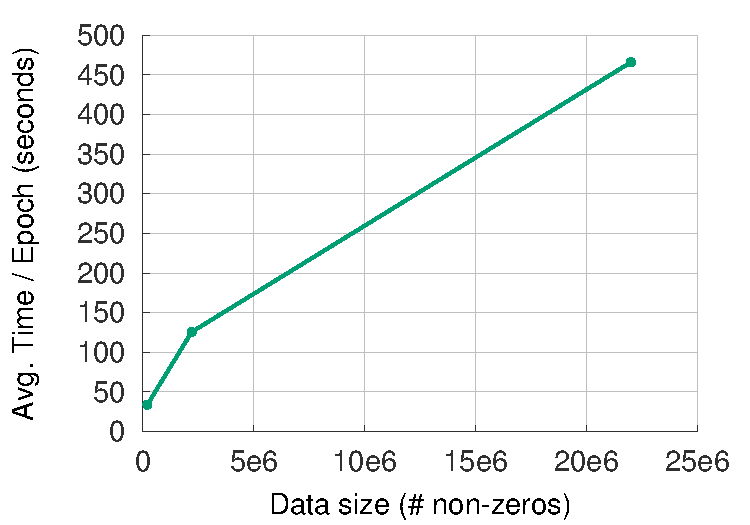
\includegraphics[width=0.5\textwidth]{fig/synth.pdf}
%  \end{center}
%  \caption{\small Scalability plot for synthetic topic model data}
%\label{fig:scalability}
%\end{figure}

%\paragraph{Scalability experiments.}
%In Figure~\ref{fig:scalability}, we show how our algorithm scales with data
%that has increasing nonzeros (simulated from a topic model). We achive a roughly linear
%increase in runtime versus data size, demonstrating that our implementation scales linearly to
%larger datasets (without introducing additional overheads or costs due to the larger data).


%\begin{table*}[t]
%\centering
%\scriptsize
%    \setlength{\tabcolsep}{4.5pt}
%\begin{tabular}{|c|c|c|c|c|c|c|c|c|c|}
%\hline
%Topic 1 & Topic 2 & Topic 3 & Topic 4 & Topic 5 & Topic 6 & Topic 7 & Topic 8 & Topic 9 & Topic 10\\
%\hline
%micchelli & kirchoff & iris & texture & maintained & foveal & neglect & microchip & microchip & indexed \\
%phased & endmember & chou & creasing & cknn & cotterill & rho & ecc & sondik & originate \\
%alike & sander & consideration & descending & spotlight & endmember & micchelli & stabilizing & unfolded & release \\
%umli & fre & retinotopic & locate & subgoal & retinotopic & cepstrum & manifold & eeg & occurred \\
%saliencies & triangulated & falling & sociated & treatment & easiest & interference & anton & shortest & multicollinearity \\
%spotlight & sep & pca & perceptual & robot & bbn & indiveri & tour & resembling & multitask \\
%gammon & assumption & eval & saund & hitting & chi & sharpe & unconditional & inhibition & dendritic \\
%sdti & hole & winner & onset & normalization & lesson & leaning & reside & cell & helpful \\
%viewer & suzanna & segmentation & lrta & fish & refractory & packet & patient & nearest & depth \\
%riken & denote & cole & mary & searching & chip & sensitivity & arethor & neighbor & partic \\
%\hline
%\end{tabular}
%\caption{\small A selection of topics from the NIPS corpus.
%}
%\label{tab:nips_lda}
%\end{table*}

%\subsubsection*{Acknowledgements}

{
\small
\bibliography{biblio}
\bibliographystyle{plain}
}

\end{document}
